\section{引\quad 言}
火星探测器气动捕获的整体制动过程如图\ref{figIntroSketch}所示。
飞行器首先由$A$点沿双曲线轨道进入火星大气,
从$A$到$B$点为气动飞行轨道段,
气动捕获制导的任务就是在此期间通过改变控制量利用气动力实现减速,
当飞行器从$B$点飞出大气后需要形成环绕轨道,
若$AB$段气动捕获任务不成功,飞行器将继续沿某条双曲线轨道飞离火星,
或飞行器没有飞出大气层,直接撞向火星地面。
成功环绕后所形成的椭圆轨道称为过渡轨道,
图中用虚线表示,该轨道的近拱点位于火星大气范围内。
然后当飞行器沿过渡轨道飞至远拱点时(图中$C$点),
需要点火加速将近拱点抬升出大气影响范围。
当飞行器再次抵近拱点时(图中$D$点),
可再次进行轨道机动调整远拱点。\cite{dqingyuan2019}
\begin{center}
	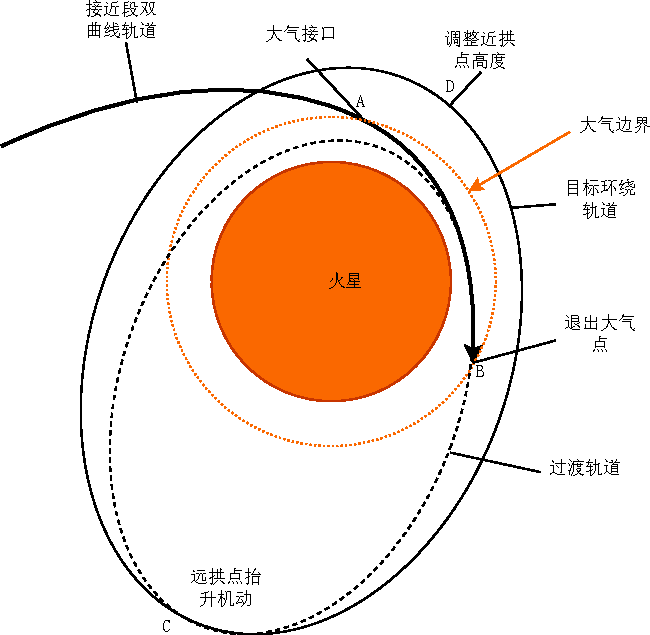
\includegraphics[scale=0.8]{IntroSketch.pdf}  \\
	\figcaption{气动捕获过程示意图} \label{figIntroSketch}
\end{center}

气动捕获制导的总体思路是,
通过不断预测以当前控制量飞出大气后的过渡轨道状态向量与目标轨道的状态向量间的误差,
代入制导算法来产生新的控制量,
如此往复,直到满足终端需求为止\cite{dqingyuan2019}。

气动捕获采用倾侧角作为控制量而不是攻角的原因有两个,
一是适用于无人任务的钝头体飞行器在气动飞行过程中所受的主轴轴向气动力远远大于其他轴所受的气动力,
控制攻角所需的力较大,需要喷气姿态发动机协助控制,同样需要消耗部分燃料。
二是攻角变化幅度过大会影响飞行器的热控能力,
因此制导算法中只有倾侧角$\sigma$为控制量,
假设攻角$\alpha$通过姿态稳定系统保持在配平攻角附近。
